\subsection{Schema generale: addestramento degli algoritmi di predizione con applicativo esterno con estensioni}
\begin{figure}[H]
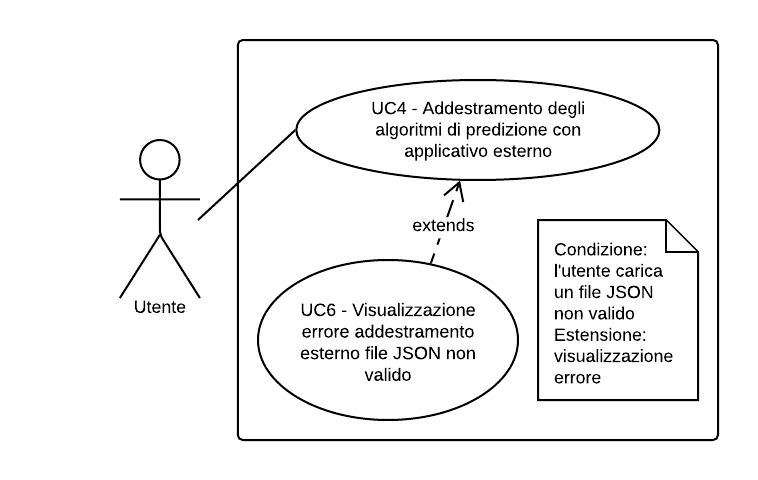
\includegraphics{img/UC4 - Schema generale.png}
\caption{Schema generale: addestramento degli algoritmi di predizione con applicativo esterno con estensioni}
\end{figure}
\subsection{UC4 - Addestramento degli algoritmi di predizione con applicativo esterno}
\begin{figure}[H]
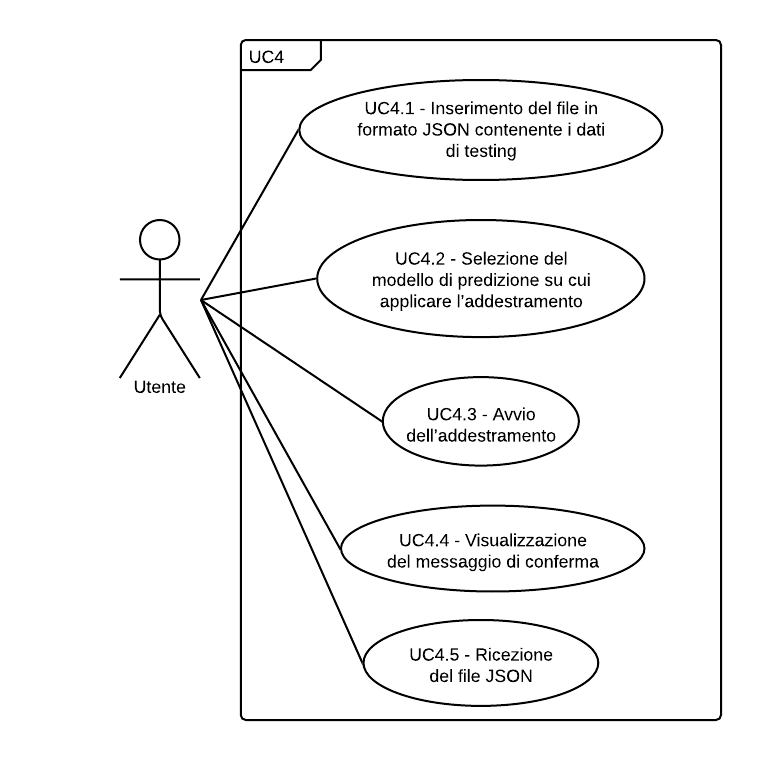
\includegraphics{img/UC4 - Addestramento degli algoritmi di predizione con applicativo esterno.png}
\caption{Diagramma degli use case di UC4}
\end{figure}
\begin{itemize}
    \item \textbf{Codice identificativo}: UC4;
    \item \textbf{Titolo}: addestramento degli algoritmi di predizione con applicativo esterno;
    \item \textbf{Attori primari}: utente;
    \item \textbf{Descrizione}: attività di addestramento degli algoritmi di predizione eseguita nell'applicativo esterno a Grafana\glosp utilizzando dei dati inseriti da un utente;
    \item \textbf{Precondizioni}: l'utente è autenticato nel sistema software Grafana\glo;
    \item \textbf{Postcondizioni}: l'utente ha completato l'addestramento degli algoritmi di predizione;
    \item \textbf{Scenario principale}: 
        \begin{enumerate}
            \item inserimento del file in formato JSON contenente i dati di testing (UC4.1);
            \item selezione del modello di predizione su cui applicare l'addestramento (UC4.2);
            \item avvio dell'addestramento (UC4.3);
            \item conclusione dell'addestramento (UC4.4);
            \item ricezione del file JSON (UC4.5). 
        \end{enumerate}
    \item \textbf{Estensioni}:
    \begin{itemize}
    	\item se il caricamento del file JSON non è avvenuto con successo viene visualizzato un messaggio di errore (UC6).
    \end{itemize}
\end{itemize}

\subsubsection{UC4.1 - Inserimento del file in formato JSON contenente i dati di testing}
\begin{figure}[H]
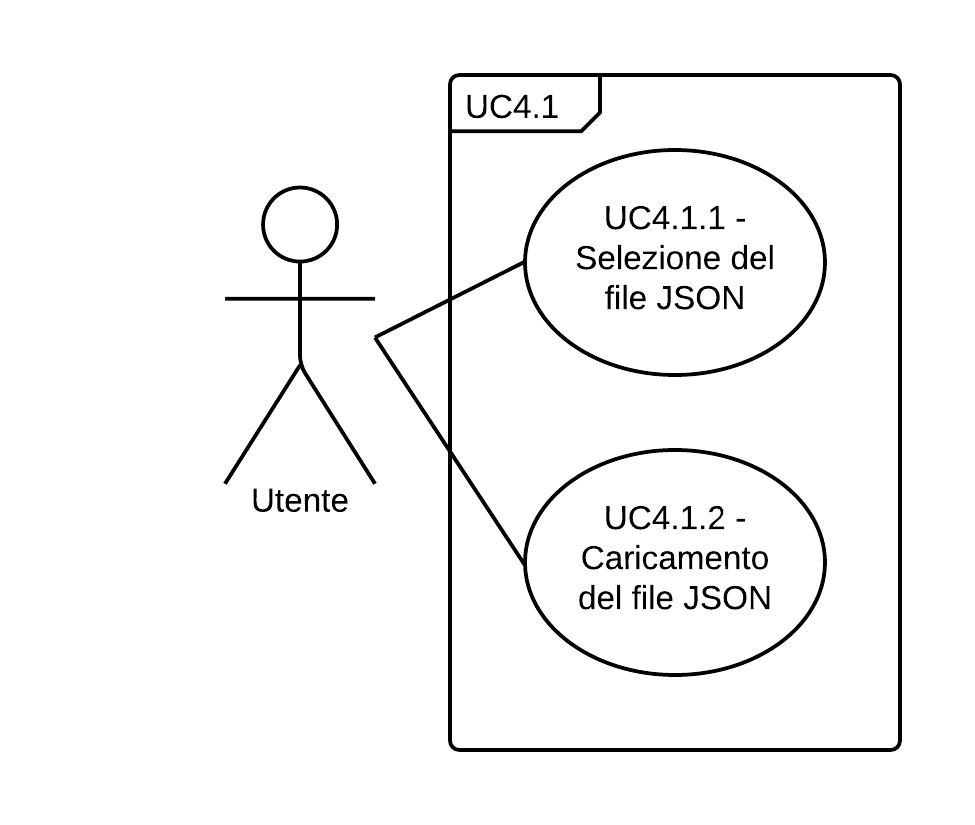
\includegraphics{img/UC4_1_-_Inserimento_del_file_in_formato_JSON_contenente_i_dati_di_testing.png}
\caption{Diagramma degli use case di UC4.1}
\end{figure}
\begin{itemize}
    \item \textbf{Codice identificativo}: UC4.1;
    \item \textbf{Titolo}: inserimento del file in formato JSON contenente i dati di testing;
    \item \textbf{Attori primari}: utente;
    \item \textbf{Descrizione}: l'utente inserisce un file in formato JSON contenente i dati di testing nell'applicazione esterna;
    \item \textbf{Precondizioni}: l'utente è autenticato nel sistema software Grafana\glo;
    \item \textbf{Postcondizioni}: l'utente ha inserito correttamente il file JSON;
    \item \textbf{Scenario principale}:
		\begin{enumerate}
			\item selezione del file JSON (UC4.1.1);
			\item caricamento del file JSON (UC4.1.2).
		\end{enumerate}
\end{itemize}

\paragraph{UC4.1.1 - Selezione del file JSON}
\begin{itemize}
	\item \textbf{Codice identificativo}: UC4.1.1;
	\item \textbf{Titolo}: selezione del file JSON;
	\item \textbf{Attori primari}: utente;
	\item \textbf{Descrizione}: l'utente seleziona il file JSON da inserire nell'applicativo esterno;
	\item \textbf{Precondizioni}: l'utente è autenticato nel sistema software Grafana\glo;
	\item \textbf{Postcondizioni}: l'utente ha selezionato correttamente il file JSON;
	\item \textbf{Scenario principale}: l'utente seleziona il file JSON.
\end{itemize}

\paragraph{UC4.1.2 - Caricamento del file JSON}
\begin{itemize}
	\item \textbf{Codice identificativo}: UC4.1.2;
	\item \textbf{Titolo}: caricamento del file JSON;
	\item \textbf{Attori primari}: utente;
	\item \textbf{Descrizione}: l'utente carica il file JSON nell'applicativo esterno;
	\item \textbf{Precondizioni}: l'utente ha selezionato il file da caricare;
	\item \textbf{Postcondizioni}: ò'utente ha caricato correttamente i file JSON;
	\item \textbf{Scenario principale}: l'utente carica il file JSON.
\end{itemize}

\subsubsection{UC4.2 - Selezione del modello di predizione su cui applicare l'addestramento}
\begin{itemize}
    \item \textbf{Codice identificativo}: UC4.2;
    \item \textbf{Titolo}: selezione del modello di predizione su cui applicare l'addestramento;
    \item \textbf{Attori primari}: utente;
    \item \textbf{Descrizione}: l'utente seleziona quale modello di predizione applicare durante l'addestramento;
    \item \textbf{Precondizioni}: il file JSON è stato inserito correttamente;
    \item \textbf{Postcondizioni}: il modello di predizione è stato scelto correttamente;
    \item \textbf{Scenario principale}: l'utente seleziona un modello di predizione per eseguire l'addestramento.   
\end{itemize}

\subsubsection{UC4.3 - Avvio dell'addestramento}
\begin{itemize}
    \item \textbf{Codice identificativo}: UC4.3;
    \item \textbf{Titolo}: avvio dell'addestramento;
    \item \textbf{Attori primari}: utente;
    \item \textbf{Descrizione}: viene fornito all'utente un modo per avviare l'addestramento;
    \item \textbf{Precondizioni}: il file JSON è stato inserito correttamente e il modello di predizione è stato selezionato;
    \item \textbf{Postcondizioni}: l'addestramento è stato avviato con successo;
    \item \textbf{Scenario principale}: l'utente avvia l'addestramento.
\end{itemize}

\paragraph{UC4.4 - Visualizzazione del messaggio di conferma}
\begin{itemize}
	\item \textbf{Codice identificativo}: UC4.4;
	\item \textbf{Titolo}: visualizzazione del messaggio di conferma;
	\item \textbf{Attori primari}: utente;
	\item \textbf{Descrizione}: l'utente visualizza un messaggio di conferma che l'addestramento è stato eseguito correttamente;
	\item \textbf{Precondizioni}: l'addestramento è stato avviato con successo;
	\item \textbf{Postcondizioni}: l'utente ha visualizzato un messaggio di conferma che l'addestramento è stato eseguito correttamente;
	\item \textbf{Scenario principale}: l'utente visualizza un messaggio di conferma che l'addestramento è stato eseguito correttamente.
\end{itemize}


\paragraph{UC4.5 - Ricezione del file JSON}
\begin{itemize}
    \item \textbf{Codice identificativo}: UC4.5;
    \item \textbf{Titolo}: ricezione del file JSON;
    \item \textbf{Attori primari}: utente;
    \item \textbf{Descrizione}: l'applicazione restituisce un file JSON con l'addestramento dei dati completato;
    \item \textbf{Precondizioni}: l'applicazione esterna ha concluso l'addestramento con successo;
    \item \textbf{Postcondizioni}: l'utente ha ricevuto il file JSON dei risultati dell'addestramento;
    \item \textbf{Scenario principale}: l'utente riceve il file JSON dei risultati dell'addestramento.
\end{itemize}